%-*- coding: UTF-8 -*-
% 1.4.tex 练习 1.4
% 勾股定理
\documentclass[nofonts]{ctexart}
\usepackage{graphicx}
\usepackage{float}
\usepackage{amsmath}
\usepackage{geometry}
\geometry{a6paper, centering, scale=0.8}
% 设置中文默认字体
\setCJKmainfont[ItalicFont={AR PL UKai CN}]{AR PL UMing CN}
% 设置文泉驿正黑字体作为中文无衬线字体
\setCJKsansfont{WenQuanYi Zen Hei}
% 设置文泉驿等宽正黑字体作为中文打字机字体
\setCJKmonofont{WenQuanYi Zen Hei Mono}

\newtheorem{thm}{定理}

\title{杂谈勾股定理}
\author{张三}
\date{\today}
\bibliographystyle{plain}

\begin{document}

\maketitle

\begin{abstract}
	这是一篇关于勾股定理的小短文.
\end{abstract}

\tableofcontents
\section{勾股定理在古代}\label{se:oldage}
西方称勾股定理为毕达哥拉斯定理, 将勾股定理的发现归功于公元前 6 世纪的
毕达哥拉斯学派\cite{Kline}. 该学派得到了一个法则, 可以求出可排成直角三角形三边的三
元数组. 毕达哥拉斯学派没有书面著作, 将定理的严格表述和证明则见于欧几里
德\footnote{欧几里德, 约公元前 330--275}《几何原本》的命题 47: 直角三
角形斜边上的正方形等于两直角边上的两个
正方形之和. 证明是用面积做的.

我国《周髀算经》载商高(约公元前 12 世纪)答周公问:
\begin{quote}
	\zihao{-5} 勾广三, 股修四, 径隅五.
\end{quote}
又载陈子(约公元前 7--6 世纪)答荣方问:

\begin{quote}
若求邪者至日者, 以日下为勾, 日高为股, 勾股各自乘, 并而开方除之, 得邪
至日.
\end{quote}

都较古希腊更早. 后者已经明确道出勾股定理的一般形式. 图\ref{fig:xiantu}
是我国古代对 勾股定理的一种证明\cite{quanjing}.
\begin{figure}[ht]
	\centering
	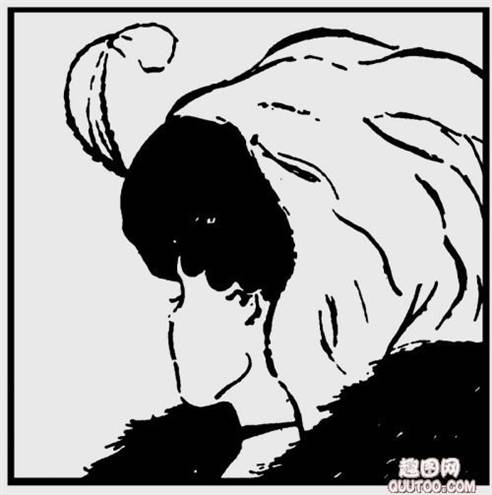
\includegraphics[scale=0.6]{lady.jpg}
	\caption{宋赵爽在《周髀算经》注中作的弦图(仿制), 该图给出了勾股
	定理的一个极具对称美的证明.}
	\label{fig:xiantu}
\end{figure}

\section{勾股定理的近代形式}
勾股定理可以用现代语言表述如下:
\begin{thm}[勾股定理]
直角三角形斜边的平方等于两腰的平方和.

可以用符号语言表述为: 设直角三角形 $ABC$, 其中$\angle C = 90^\circ$, 则有
\begin{equation}
	AB^2 = BC^2 + AC^2
	\label{eq:gougu}
\end{equation}
\end{thm}
满足式子\eqref{eq:gougu}的整数称为\emph{勾股数}. 第 \ref{se:oldage}
节所说毕达哥拉斯学派得到的三元数组就是
勾股数. 下表列出了一些较小的勾股数:
\begin{table}[H]
\begin{tabular}{|rrr|}
	\hline
	直角边	$a$ & 直角边 $b$ & 斜边 $c$ \\
	\hline
	3	    &	4  	 & 5	    \\
	5	    &   12       & 13       \\
	\hline
\end{tabular}%
\qquad
($a^2+b^2=c^2$)
\end{table}

\nocite{Shiye}
\bibliography{math}

\end{document}
